\documentclass[10pt,a4paper]{article}

\usepackage[spanish,activeacute,es-tabla]{babel}
\usepackage[utf8]{inputenc}
\usepackage{ifthen}
\usepackage{listings}
\usepackage{dsfont}
\usepackage{subcaption}
\usepackage{amsmath}
\usepackage[strict]{changepage}
\usepackage[top=1cm,bottom=2cm,left=1cm,right=1cm]{geometry}%
\usepackage{color}%
\newcommand{\tocarEspacios}{%
	\addtolength{\leftskip}{3em}%
	\setlength{\parindent}{0em}%
}

% Especificacion de procs

\newcommand{\In}{\textsf{in }}
\newcommand{\Out}{\textsf{out }}
\newcommand{\Inout}{\textsf{inout }}

\newcommand{\encabezadoDeProc}[4]{%
	% Ponemos la palabrita problema en tt
	%  \noindent%
	{\normalfont\bfseries\ttfamily proc}%
	% Ponemos el nombre del problema
	\ %
	{\normalfont\ttfamily #2}%
	\
	% Ponemos los parametros
	(#3)%
	\ifthenelse{\equal{#4}{}}{}{%
		% Por ultimo, va el tipo del resultado
		\ : #4}
}

\newenvironment{proc}[4][res]{%
	
	% El parametro 1 (opcional) es el nombre del resultado
	% El parametro 2 es el nombre del problema
	% El parametro 3 son los parametros
	% El parametro 4 es el tipo del resultado
	% Preambulo del ambiente problema
	% Tenemos que definir los comandos requiere, asegura, modifica y aux
	\newcommand{\requiere}[2][]{%
		{\normalfont\bfseries\ttfamily requiere}%
		\ifthenelse{\equal{##1}{}}{}{\ {\normalfont\ttfamily ##1} :}\ %
		\{\ensuremath{##2}\}%
		{\normalfont\bfseries\,\par}%
	}
	\newcommand{\asegura}[2][]{%
		{\normalfont\bfseries\ttfamily asegura}%
		\ifthenelse{\equal{##1}{}}{}{\ {\normalfont\ttfamily ##1} :}\
		\{\ensuremath{##2}\}%
		{\normalfont\bfseries\,\par}%
	}
	\renewcommand{\aux}[4]{%
		{\normalfont\bfseries\ttfamily aux\ }%
		{\normalfont\ttfamily ##1}%
		\ifthenelse{\equal{##2}{}}{}{\ (##2)}\ : ##3\, = \ensuremath{##4}%
		{\normalfont\bfseries\,;\par}%
	}
	\renewcommand{\pred}[3]{%
		{\normalfont\bfseries\ttfamily pred }%
		{\normalfont\ttfamily ##1}%
		\ifthenelse{\equal{##2}{}}{}{\ (##2) }%
		\{%
		\begin{adjustwidth}{+5em}{}
			\ensuremath{##3}
		\end{adjustwidth}
		\}%
		{\normalfont\bfseries\,\par}%
	}
	
	\newcommand{\res}{#1}
	\vspace{1ex}
	\noindent
	\encabezadoDeProc{#1}{#2}{#3}{#4}
	% Abrimos la llave
	\par%
	\tocarEspacios
}
{
	% Cerramos la llave
	\vspace{1ex}
}

\newcommand{\aux}[4]{%
	{\normalfont\bfseries\ttfamily\noindent aux\ }%
	{\normalfont\ttfamily #1}%
	\ifthenelse{\equal{#2}{}}{}{\ (#2)}\ : #3\, = \ensuremath{#4}%
	{\normalfont\bfseries\,;\par}%
}

\newcommand{\pred}[3]{%
	{\normalfont\bfseries\ttfamily\noindent pred }%
	{\normalfont\ttfamily #1}%
	\ifthenelse{\equal{#2}{}}{}{\ (#2) }%
	\{%
	\begin{adjustwidth}{+2em}{}
		\ensuremath{#3}
	\end{adjustwidth}
	\}%
	{\normalfont\bfseries\,\par}%
}

% Tipos

\newcommand{\nat}{\ensuremath{\mathds{N}}}
\newcommand{\ent}{\ensuremath{\mathds{Z}}}
\newcommand{\float}{\ensuremath{\mathds{R}}}
\newcommand{\bool}{\ensuremath{\mathsf{Bool}}}
\newcommand{\cha}{\ensuremath{\mathsf{Char}}}
\newcommand{\str}{\ensuremath{\mathsf{String}}}

% Logica

\newcommand{\True}{\ensuremath{\mathrm{true}}}
\newcommand{\False}{\ensuremath{\mathrm{false}}}
\newcommand{\Then}{\ensuremath{\rightarrow}}
\newcommand{\Iff}{\ensuremath{\leftrightarrow}}
\newcommand{\implica}{\ensuremath{\longrightarrow}}
\newcommand{\IfThenElse}[3]{\ensuremath{\mathsf{if}\ #1\ \mathsf{then}\ #2\ \mathsf{else}\ #3\ \mathsf{fi}}}
\newcommand{\yLuego}{\land _L}
\newcommand{\oLuego}{\lor _L}
\newcommand{\implicaLuego}{\implica _L}

\newcommand{\cuantificador}[5]{%
	\ensuremath{(#2 #3: #4)\ (%
		\ifthenelse{\equal{#1}{unalinea}}{
			#5
		}{
			$ % exiting math mode
			\begin{adjustwidth}{+2em}{}
				$#5$%
			\end{adjustwidth}%
			$ % entering math mode
		}
		)}
}

\newcommand{\existe}[4][]{%
	\cuantificador{#1}{\exists}{#2}{#3}{#4}
}
\newcommand{\paraTodo}[4][]{%
	\cuantificador{#1}{\forall}{#2}{#3}{#4}
}

%listas

\newcommand{\TLista}[1]{\ensuremath{seq \langle #1\rangle}}
\newcommand{\lvacia}{\ensuremath{[\ ]}}
\newcommand{\lv}{\ensuremath{[\ ]}}
\newcommand{\longitud}[1]{\ensuremath{|#1|}}
\newcommand{\cons}[1]{\ensuremath{\mathsf{addFirst}}(#1)}
\newcommand{\indice}[1]{\ensuremath{\mathsf{indice}}(#1)}
\newcommand{\conc}[1]{\ensuremath{\mathsf{concat}}(#1)}
\newcommand{\cab}[1]{\ensuremath{\mathsf{head}}(#1)}
\newcommand{\cola}[1]{\ensuremath{\mathsf{tail}}(#1)}
\newcommand{\sub}[1]{\ensuremath{\mathsf{subseq}}(#1)}
\newcommand{\en}[1]{\ensuremath{\mathsf{en}}(#1)}
\newcommand{\cuenta}[2]{\mathsf{cuenta}\ensuremath{(#1, #2)}}
\newcommand{\suma}[1]{\mathsf{suma}(#1)}
\newcommand{\twodots}{\ensuremath{\mathrm{..}}}
\newcommand{\masmas}{\ensuremath{++}}
\newcommand{\matriz}[1]{\TLista{\TLista{#1}}}
\newcommand{\seqchar}{\TLista{\cha}}

\renewcommand{\lstlistingname}{Código}
\lstset{% general command to set parameter(s)
	language=Java,
	morekeywords={endif, endwhile, skip},
	basewidth={0.47em,0.40em},
	columns=fixed, fontadjust, resetmargins, xrightmargin=5pt, xleftmargin=15pt,
	flexiblecolumns=false, tabsize=4, breaklines, breakatwhitespace=false, extendedchars=true,
	numbers=left, numberstyle=\tiny, stepnumber=1, numbersep=9pt,
	frame=l, framesep=3pt,
	captionpos=b,
}

\usepackage{caratula} % Version modificada para usar las macros de algo1 de ~> https://github.com/bcardiff/dc-tex

\titulo{Trabajo Práctico 2}
\subtitulo{Clasificación y Selección de Modelos}

\fecha{\today}

\materia{Laboratorio de Datos}
\grupo{Grupo 100}

\integrante{Chapana Puma, Joselin Miriam}{1197/21}{yoselin.chapana@gmail.com}
\integrante{Martinelli, Lorenzo}{364/23}{martinelli.lorenzo12@gmail.com}
\integrante{Padilla, Ramiro}{1636/21}{ramiromdq123@gmail.com}
% Pongan cuantos integrantes quieran

% Declaramos donde van a estar las figuras
% No es obligatorio, pero suele ser comodo
\graphicspath{{../static/}}

\begin{document}
\maketitle

\section{Introducción}  \vspace{0.1cm}

\subsection{Fuente de datos} \vspace{0.2cm}

A lo largo de este proyecto, trabajaremos con un conjunto de datos de imágenes denominado Sign
Language MNIST\footnote{Link al dataset https://www.kaggle.com/datasets/datamunge/sign-language-mnist}, el cual se encuentra en formato csv, donde cada imagen del set de datos representa una letra en lenguaje de señas americano. El link al dataset se encuentra al pie de página.

\subsection{Análisis exploratorio de datos}  \vspace{0.2cm}

Antes de ponernos a trabajar con los datos, necesitamos saber mas acerca de ellos. Sabemos que, cada fila del dataset representa una imagen de 28x28 pixeles en escala de grises que corresponde a una letra en lenguaje de señas. Miremos a continuación un pequeño fragmento del mismo. En este, podremos ver las semejanzas y diferencias que tenemos entre las distintas letras. También, se puede ver en menor medida similitudes entre letras de la misma clase.

 \vspace{0.2cm}

\begin{figure}[h]
  \centering
  \includegraphics[width=1.0\textwidth]{Imagenes/atributos\_relevantes.png}
  \caption{Primeras quince imagenes del dataset}
  \label{fig:Tabla 1}
\end{figure}

 \vspace{0.2cm}

A partir del gráfico anterior, podemos inferir que no todos los pixeles son realmente relevantes para diferenciar imágenes entre si. Por ejemplo, podemos ver
que aquellos pixeles correspondientes al fondo no aportan información alguna. ¿Cuántos pixeles necesitaremos realmente para diferenciar las imágenes? \vspace{0.05cm}

Por otro lado, viendo por ejemplo, que las letras C y D aparecen más de una vez, también surge la pregunta. ¿Están balanceadas las distintas clases que identifican a las letras? En el gráfico a continuación, podremos notar que tenemos un dataset con una excelente distribución de clases. ¿Por qué me interesa
tener una cantidad pareja de cada muestra? Esto, adquiere relevancia puesto que al entrenar nuestros modelos en un futuro, no queremos tener sesgos.
\vspace{0.05cm}
  
Obs: Las letras J y Z no poseen ningún ejemplar puesto que requieren de movimiento para su seña.

\vspace{0.1cm}

\begin{figure}[h]
  \centering
  \includegraphics[width=0.8\textwidth]{Imagenes/distribucion.png}
  \caption{Cantidad de muestras de cada letra}
  \label{fig:Tabla 2}
\end{figure}

\newpage

Otra pregunta que naturalmente surge al explorar el dataset es que tan distintas son las letras entre sí, y si las diferentes muestras respecto a una misma letras
presentan diferencias notorias o no. Para eso, comparemos por ejemplo, las letras E, L y M.

\begin{figure}[ht!]
	\begin{subfigure}{0.5\textwidth}
		\includegraphics[width=1\linewidth]{Imagenes/letra\_E\_vs\_L.png} 
		\caption{Muestras de las letras E y L}
		\label{fig:subfig1}
	\end{subfigure}
	\begin{subfigure}{0.5\textwidth}
		\includegraphics[width=1\linewidth]{Imagenes/letra\_E\_vs\_M.png}
		\caption{Muestras de las letras E y M}
		\label{fig:subfig2}
	\end{subfigure}
	% OJO: el caption siempre va antes del label
	\label{fig:subfigs}
\end{figure}

En la imagen anterior, podemos apreciar que tanto la letra E como la M son muy distintas a la letra L, sin embargo, poseen muchas semenjanzas entre sí. Esto, es algo a tener en cuenta a la hora de plantear los modelos, cuales serán los pixeles mas representativos para imagenes similares.
Miremos también, si en imagenes pertenencientes a una misma letra hay diferencias notorias. 

\begin{figure}[ht!]
	\begin{subfigure}{0.5\textwidth}
		\centering
		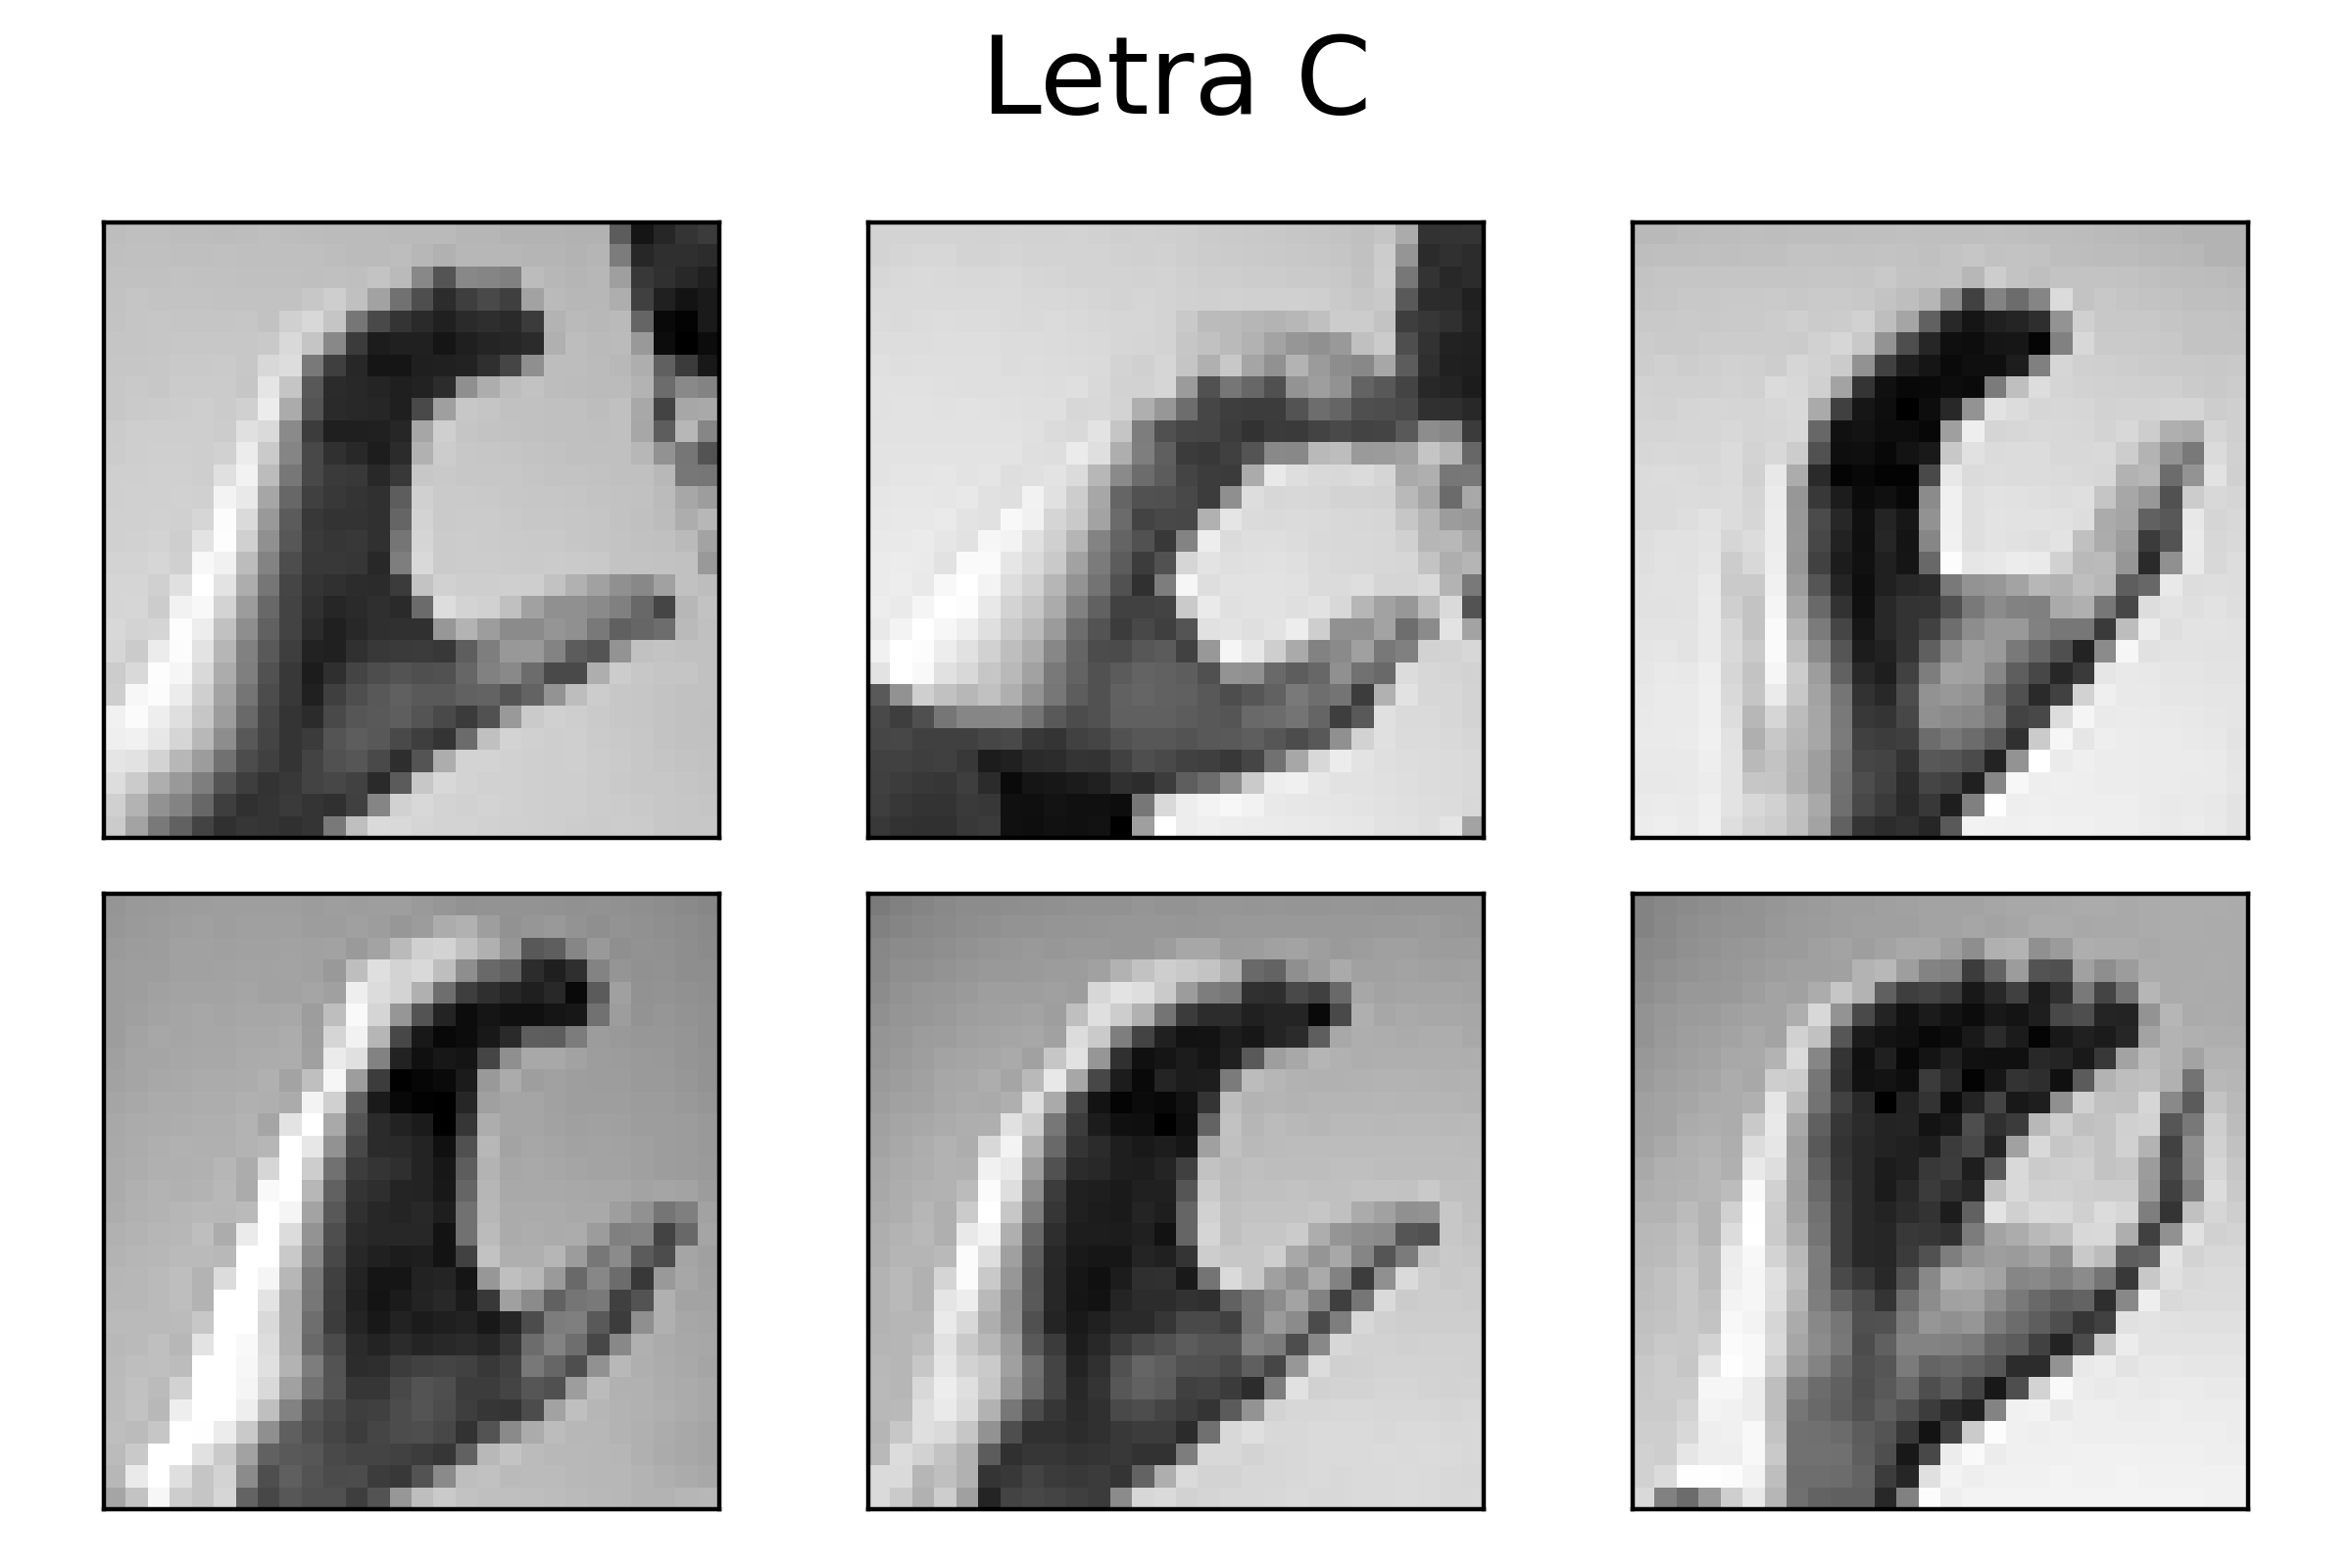
\includegraphics[width=1\linewidth]{Imagenes/letra_C.png} 
		\caption{Distintas muestras de la letra C}
		\label{fig:subfig1}
	\end{subfigure}
	\begin{subfigure}{0.55\textwidth}
		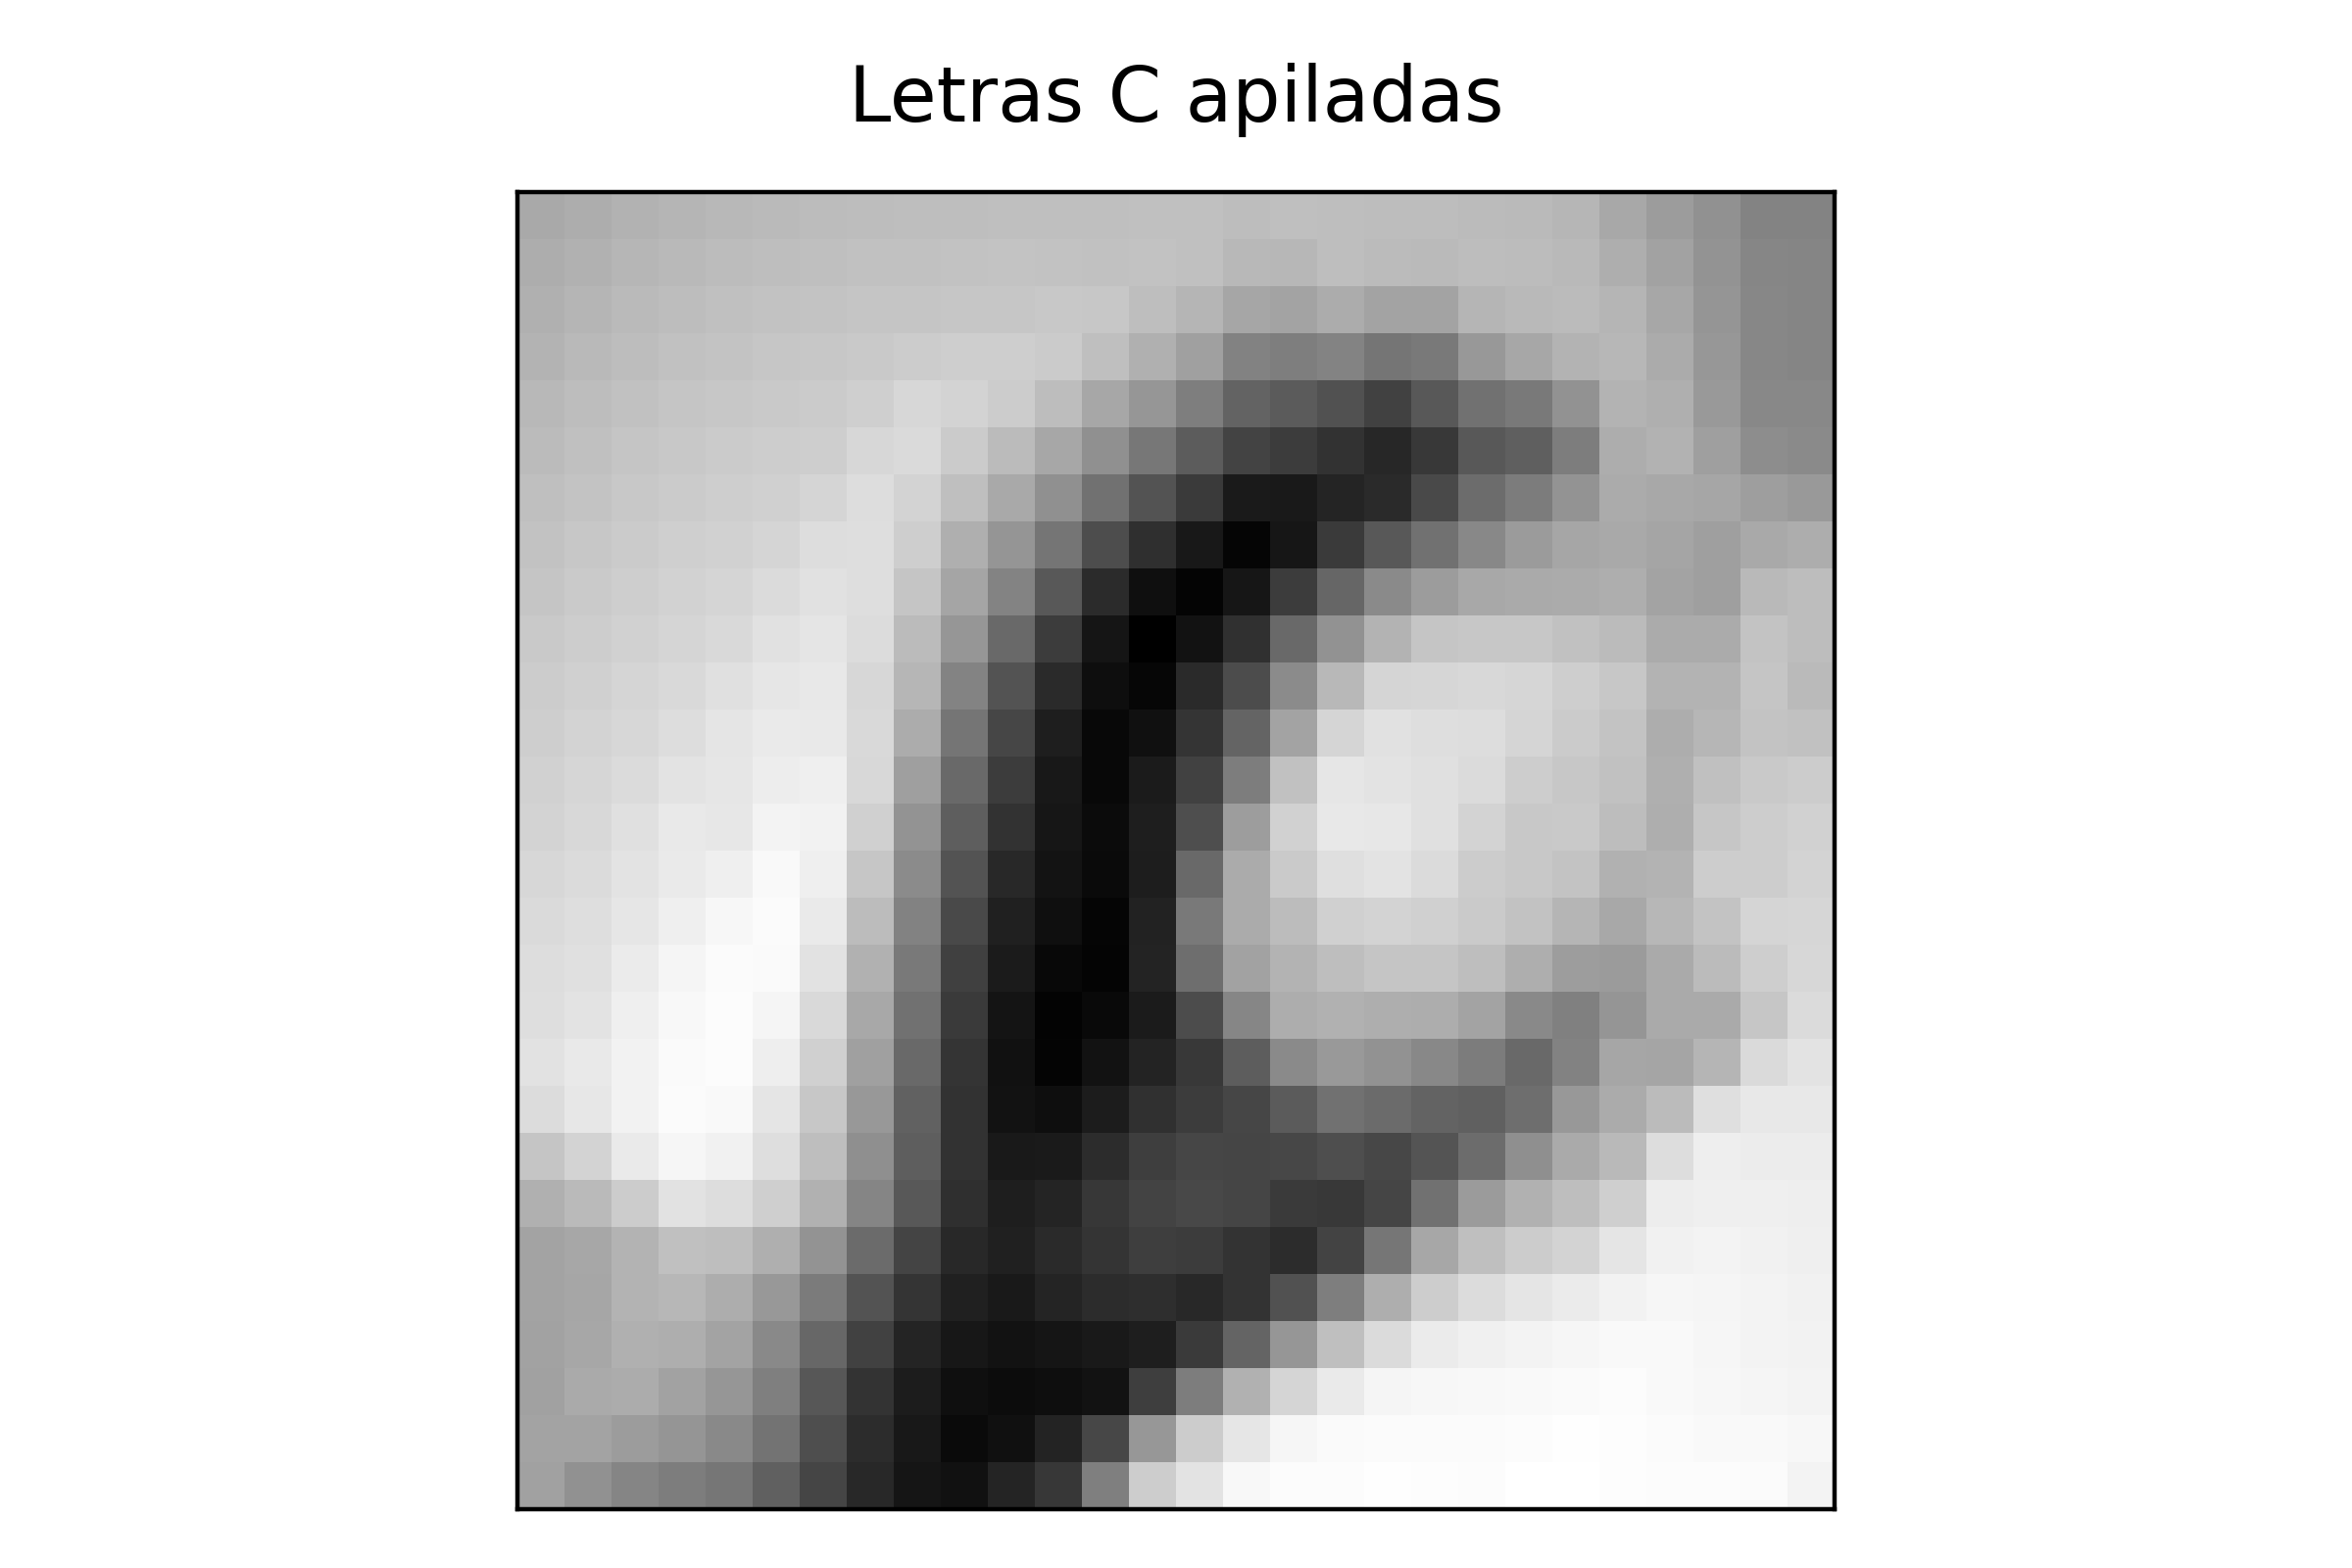
\includegraphics[width=1\linewidth]{Imagenes/letra_C_apilada.png}
		\caption{Todas las muestras de la letra C apiladas}
		\label{fig:subfig2}
	\end{subfigure}
	% OJO: el caption siempre va antes del label
	\label{fig:subfigs}
\end{figure}

\newpage

Si bien, a simple vista, cuando comparamos algunos ejemplares, pareciera que las diferencias pueden llegar a ser significativas, a la hora de comparar todos los ejemplares, en este caso, apilandolos, notamos que forman una silueta que representa muy bien la seña a la que corresponde. \vspace{0.1cm}

A partir de todo el análisis anterior, pudimos notar que no representa diferencias significativas el trabajar con imagenes respecto a datasets como el del titanic, respecto a su dificultad. Si, quizas, lleva algo mas de tiempo su análisis, pero con las herramientas indicadas no presenta mayores dificultades.

\vspace{0.1cm}


\section{Modelo}

\subsection{¿La imagen corresponde a una seña de la L o a una seña de la A?} \vspace{0.1cm}

En esta sección, trabajeremos con un subconjunto del dataset original, donde solo esten las letras A  y L. Nuestro objetivo, será encontrar un modelo que
diferencie estas letras con la menor cantidad de pixeles posibles. Comencemos entonces viendo cuantas muestras tenemos. 

\begin{figure}[h]
	\centering
  \includegraphics[width=0.5\textwidth]{Imagenes/cantidad\_letras\_A\_L.png}
  \caption{Distribución de Letras}
  \label{fig:Tabla 6}
\end{figure}

Sabemos entonces, que tenemos buena distribución lo que nos ayuda al armado de los conjuntos de train y test. Veamos ahora, las diferencias entres estas letras en la imagen a continuación.  Del lado izquierdo tenemos una comparativa entre todas letras L y las letras A apiladas, y del otro lado, tenemos la resta entre ambas, puesto que es de nuestro interes obtener las zonas de mayor varianza.

\newpage

\begin{figure}[ht!]
	\begin{subfigure}{0.5\textwidth}
		\centering
		\includegraphics[width=1\linewidth]{Imagenes/letras\_A\_L\_apiladas.png} 
		\caption{Todas las letras A y L apiladas y reescaladas}
		\label{fig:subfig1}
	\end{subfigure}
	\begin{subfigure}{0.55\textwidth}
		\includegraphics[width=1\linewidth]{Imagenes/varianza.png}
		\caption{L - A}
		\label{fig:subfig2}
	\end{subfigure}
	% OJO: el caption siempre va antes del label
	\label{fig:subfigs}
\end{figure}

Notamos que, la zona con mayor varianza seria en la zona mas oscura que aparece en el medio de la imagen o, en su defecto, la zona mas blanca. Para saber esto con precisión utilizamos una función de pandas que nos devuelve en una lista las 10 posiciones con los valores mas altos. Destacando, que los pixeles
mas representativos son el 301, 274 y 246. 

\subsection{Construcción del Modelo} \vspace{0.1cm}

Una vez, que conocemos bastante acerca de nuestro dataset, estamos en condiciones de armar nuestro clasificador Knn. A fines de afinar nuestro modelo, hicimos pruebas utilizando distintas cantidades de pixeles, la idea es, utilizar la menor cantidad posible para asi no usar datasets tan grandes. Veamos los resultados.

\begin{figure}[h]
  \centering
  \includegraphics[width=0.6\textwidth]{Imagenes/pixelesvsacc.png}
  \caption{Pixeles vs Accuracy}
  \label{fig:Tabla 1}
\end{figure}

Una observación, para tener un gráfico mas confiable, lo que hicimos fue realizar la prueba de precisión una cierta cantidad de veces, tomando en cada iteracion pixeles al azar, para luego tomar su promedio, de esta manera garantizamos cierta aleatoreidad.

\subsection{Conclusiones Clasificación Binaria}

Pudimos destacar la importancia de comenzar con un analisis exploratorio de los datos correspondientes a las letras L y A, lo que nos permitió notar y diferenciar aquellos pixeles que presentan mayor varianza entre las dos letras, para luego mejorar la performance utilizando estos atributos. Una vez hecho esto, tambien observamos que la perfomance baja al aumentar la cantidad de vecinos. Por lo tanto, podemos concluir que tomando un modelo que tenga entre 3 y 10 pixeles con alta varianza y con k = 1, tendriamos un modelo eficiente con una perfomance aproximada de $0.99$. 

\newpage

Como se puede apreciar en la imagen anterior, la precisión aumenta de manera notable a partir de los 3 pixeles para luego estabilizarse alrededor de los 7.
Veamos que ocurre ahora para algunos de estos valores si modificamos la cantidad de vecinos.

\begin{figure}[ht!]
	\begin{subfigure}{0.5\textwidth}
		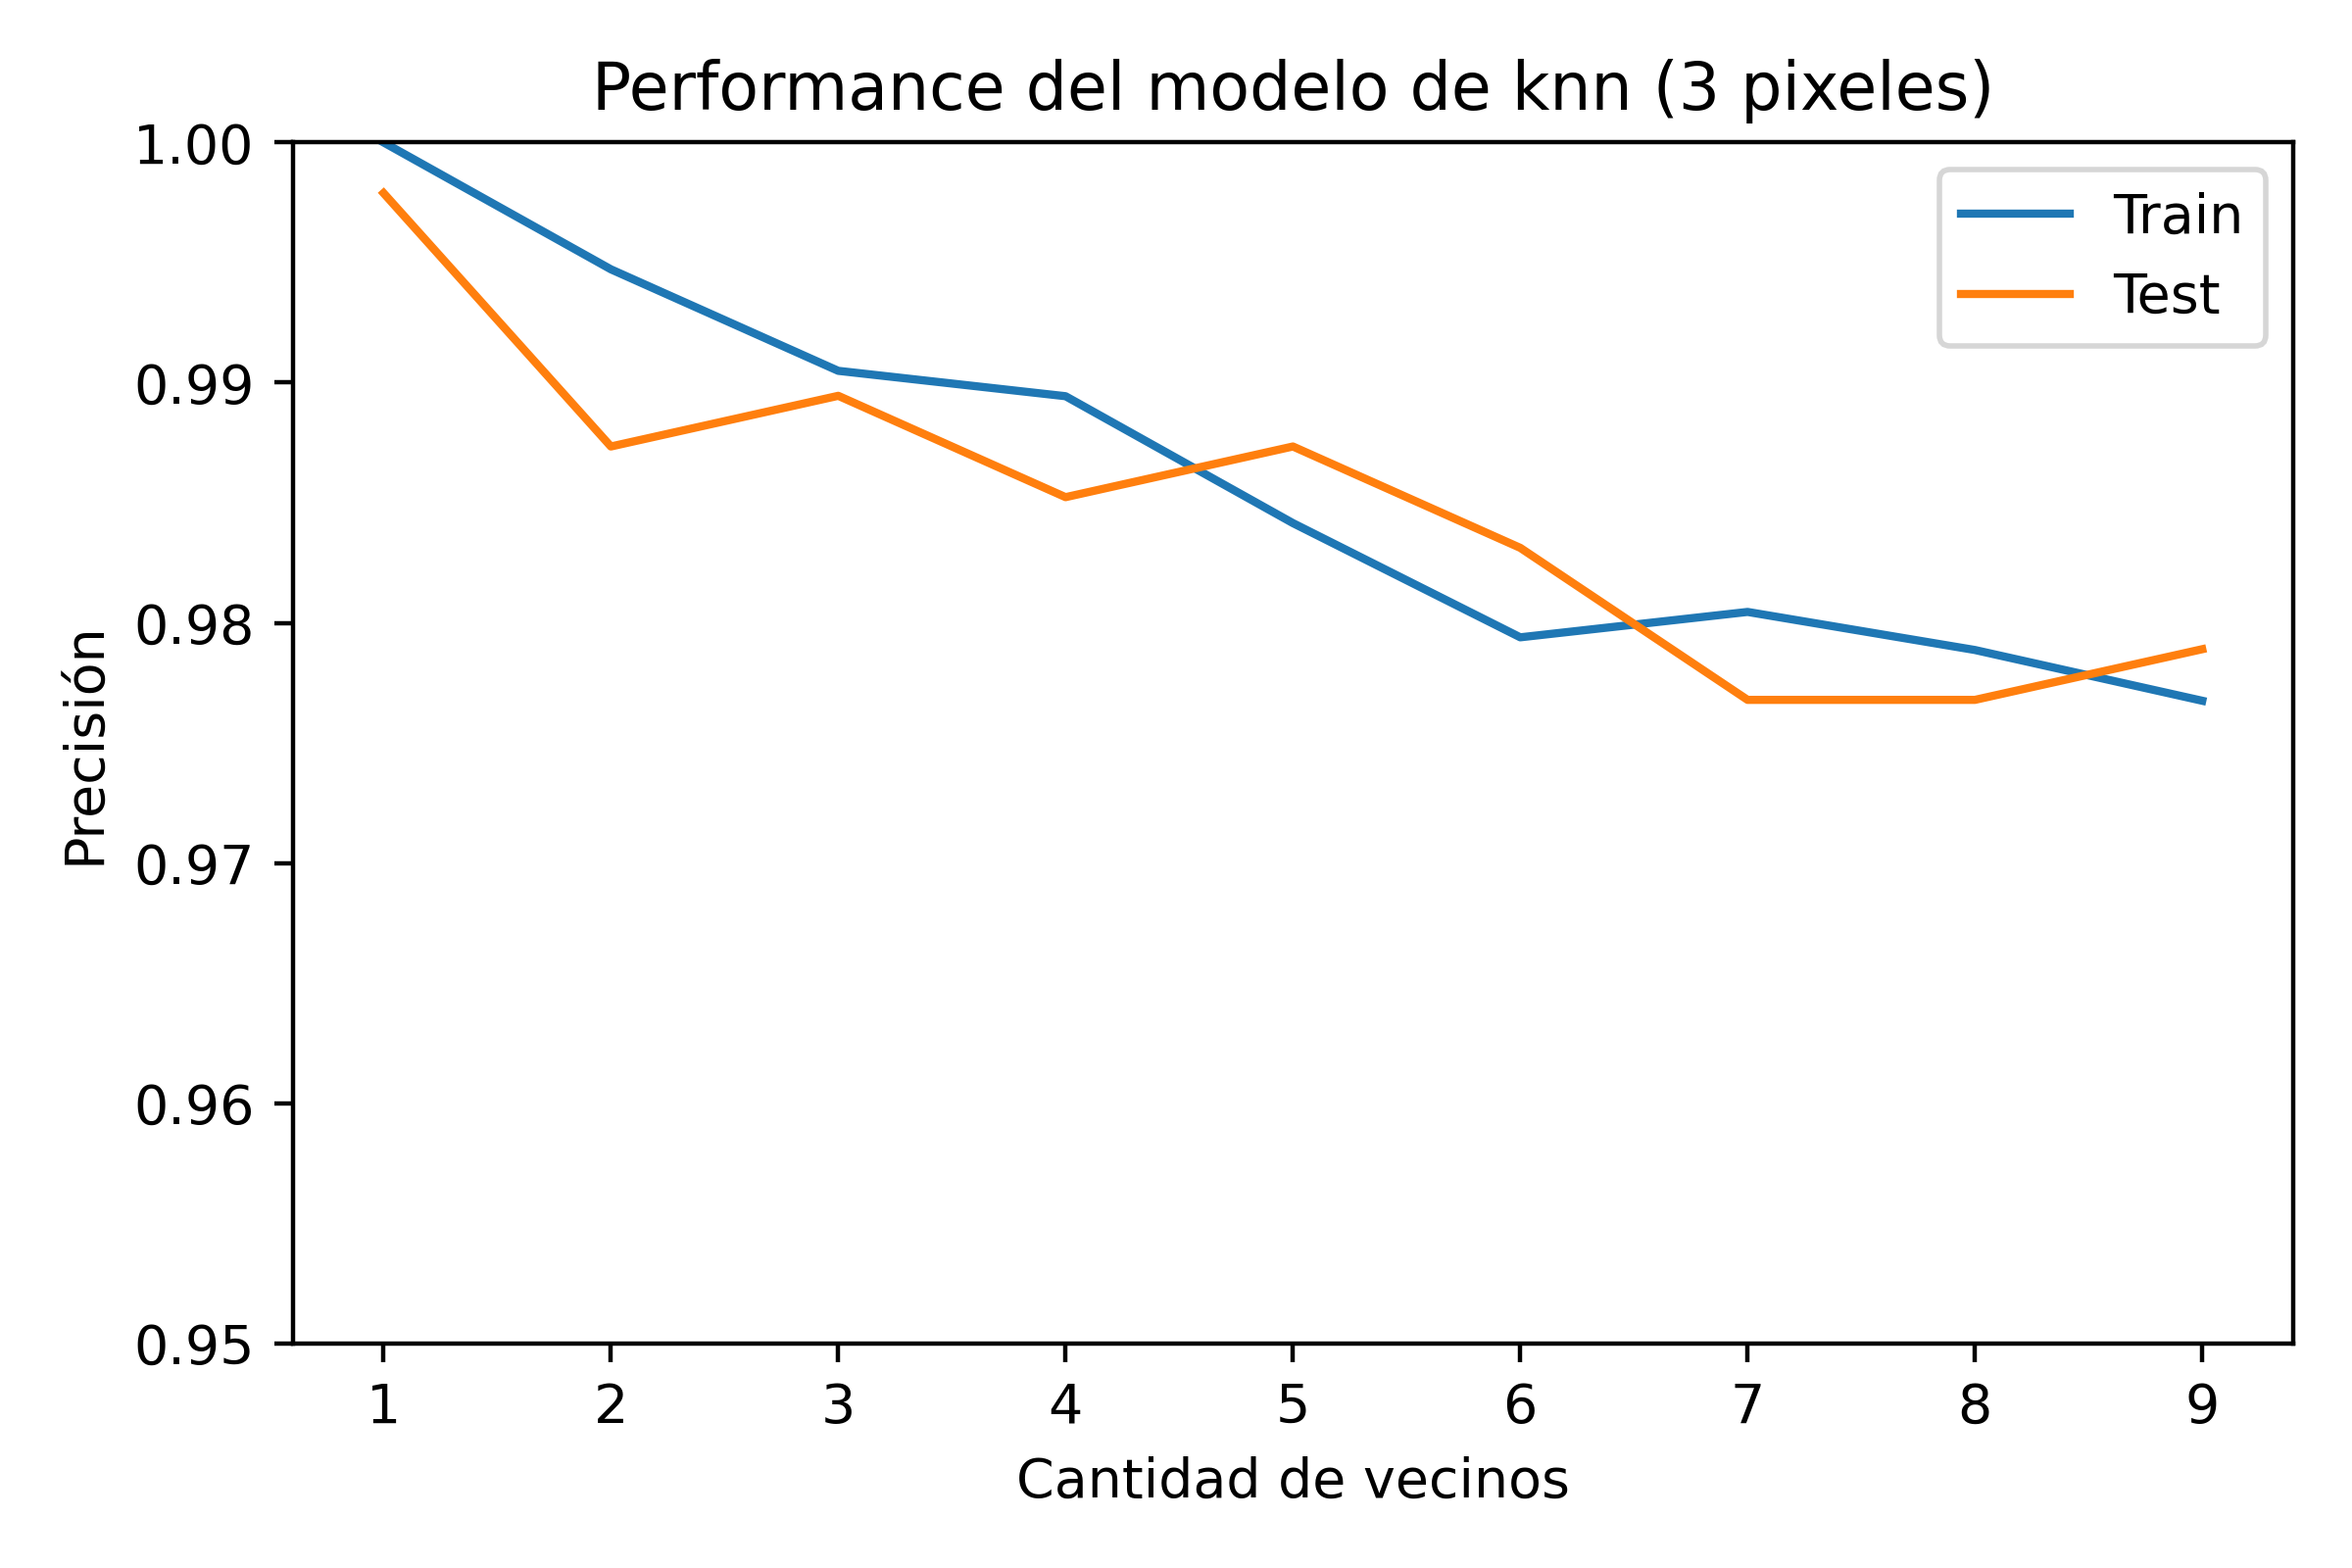
\includegraphics[width=1\linewidth]{Imagenes/3pixeles.png} 
		\caption{Pixeles mas significativos}
		\label{fig:subfig1}
	\end{subfigure}
	\begin{subfigure}{0.5\textwidth}
		\includegraphics[width=1\linewidth]{Imagenes/3pixelesRandom.png}
		\caption{Pixeles aleatorios}
		\label{fig:subfig2}
	\end{subfigure}
	% OJO: el caption siempre va antes del label
	\label{fig:subfigs}
\end{figure}

Podemos ver claramente que, contrario a lo que uno podria pensar, la performance baja a medida que tenemos mas vecinos, siendo el numero ideal exactamente 1. Notar que en estas pruebas tomamos por un lado los pixeles de mayor varianza que habiamos encontrados antes y, pixeles aleatorios.
\vspace{0.05cm}
Veamos tambien, un caso con mas pixeles a ver que ocurre

\begin{figure}[ht!]
	\begin{subfigure}{0.5\textwidth}
		\includegraphics[width=1\linewidth]{imagenes/10pixeles.png} 
		\caption{Pixeles de alta varianza}
		\label{fig:subfig1}
	\end{subfigure}
	\begin{subfigure}{0.5\textwidth}
		\includegraphics[width=1\linewidth]{Imagenes/10pixelesRandom.png}
		\caption{Pixeles aleatorios}
		\label{fig:subfig2}
	\end{subfigure}
	% OJO: el caption siempre va antes del label
	\label{fig:subfigs}
\end{figure}

Al igual que cuando testeamos la performance en función de la cantidad de atributos, cuando hicimos la prueba con 3 y 10 pixeles aleatorios, la repetimos una cierta cantidad de veces y obtuvimos su promedio, con el cual realizamos los gráficos anteriores.

\newpage

\section{Clasificador Multiclase}

\vspace{0.05cm}

\subsection{¿A cuál de las vocales corresponde la seña en la imagen?}

En esta sección, se intentará encontrar un modelo de árbol de decisión que prediga las vocales. Para esto, armaremos un dataset a partir del original el cual contenga unicamente estas. \vspace{0.05cm}

A fin de encontrar el mejor modelo, realizamos distintas pruebas modificando los paramentros del modelo. En primer lugar, lo que hicimos fue testear alturas
entre 1 y 14. Para esto, utilizamos dos métodos, por un lado dividimos  el dataset original en train, validation y test, para luego entrenar
el modelo con los datos de train y medirlo contra los datos de validation. 

\begin{figure}[h]
  \centering
  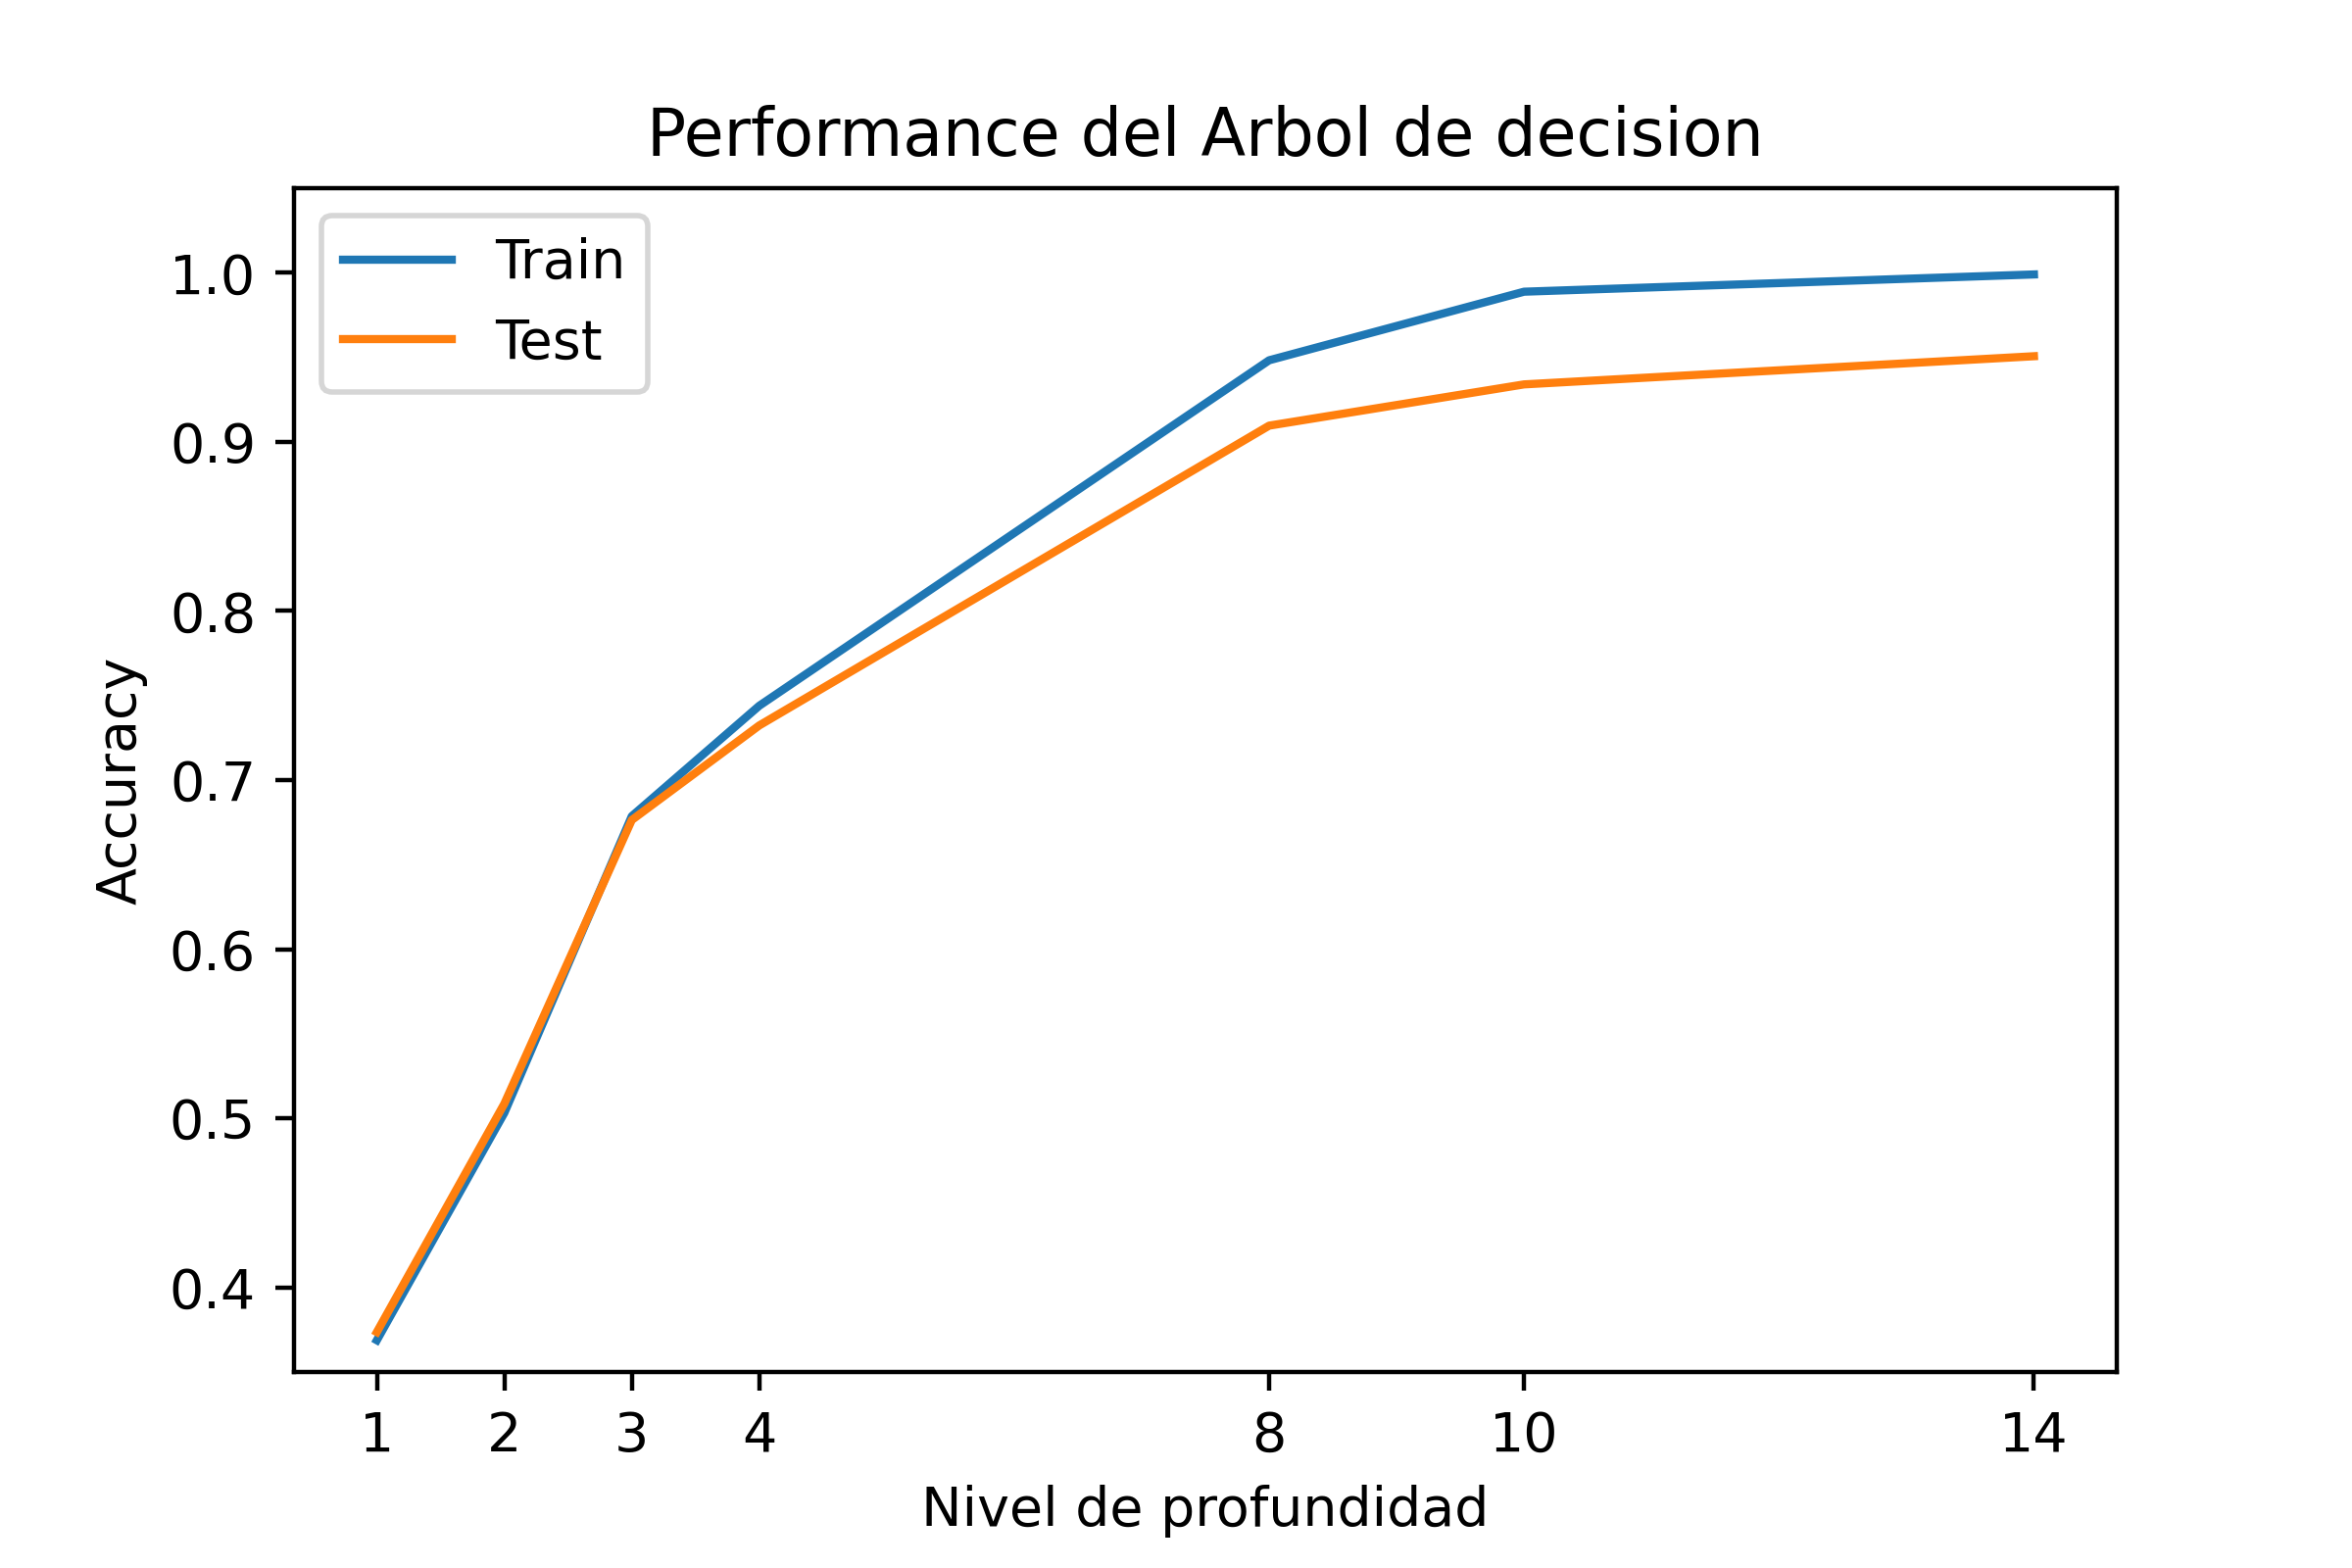
\includegraphics[width=0.6\textwidth]{Imagenes/primer_prueba_arbol.png}
  \caption{Prueba para distintas profundidades}
  \label{fig:Tabla 1}
\end{figure}

Por otro lado,para poder comparar y seleccionar el mejor árbol de decisión, se empleo validacion cruzada con k-folding utilizando los datos de train, los cuales
en este caso son la union entre los datos de train y validacion anteriores. Veamos entonces los resultados comparados con el test anterior.

\begin{figure}[ht!]
	\begin{subfigure}{0.5\textwidth}
		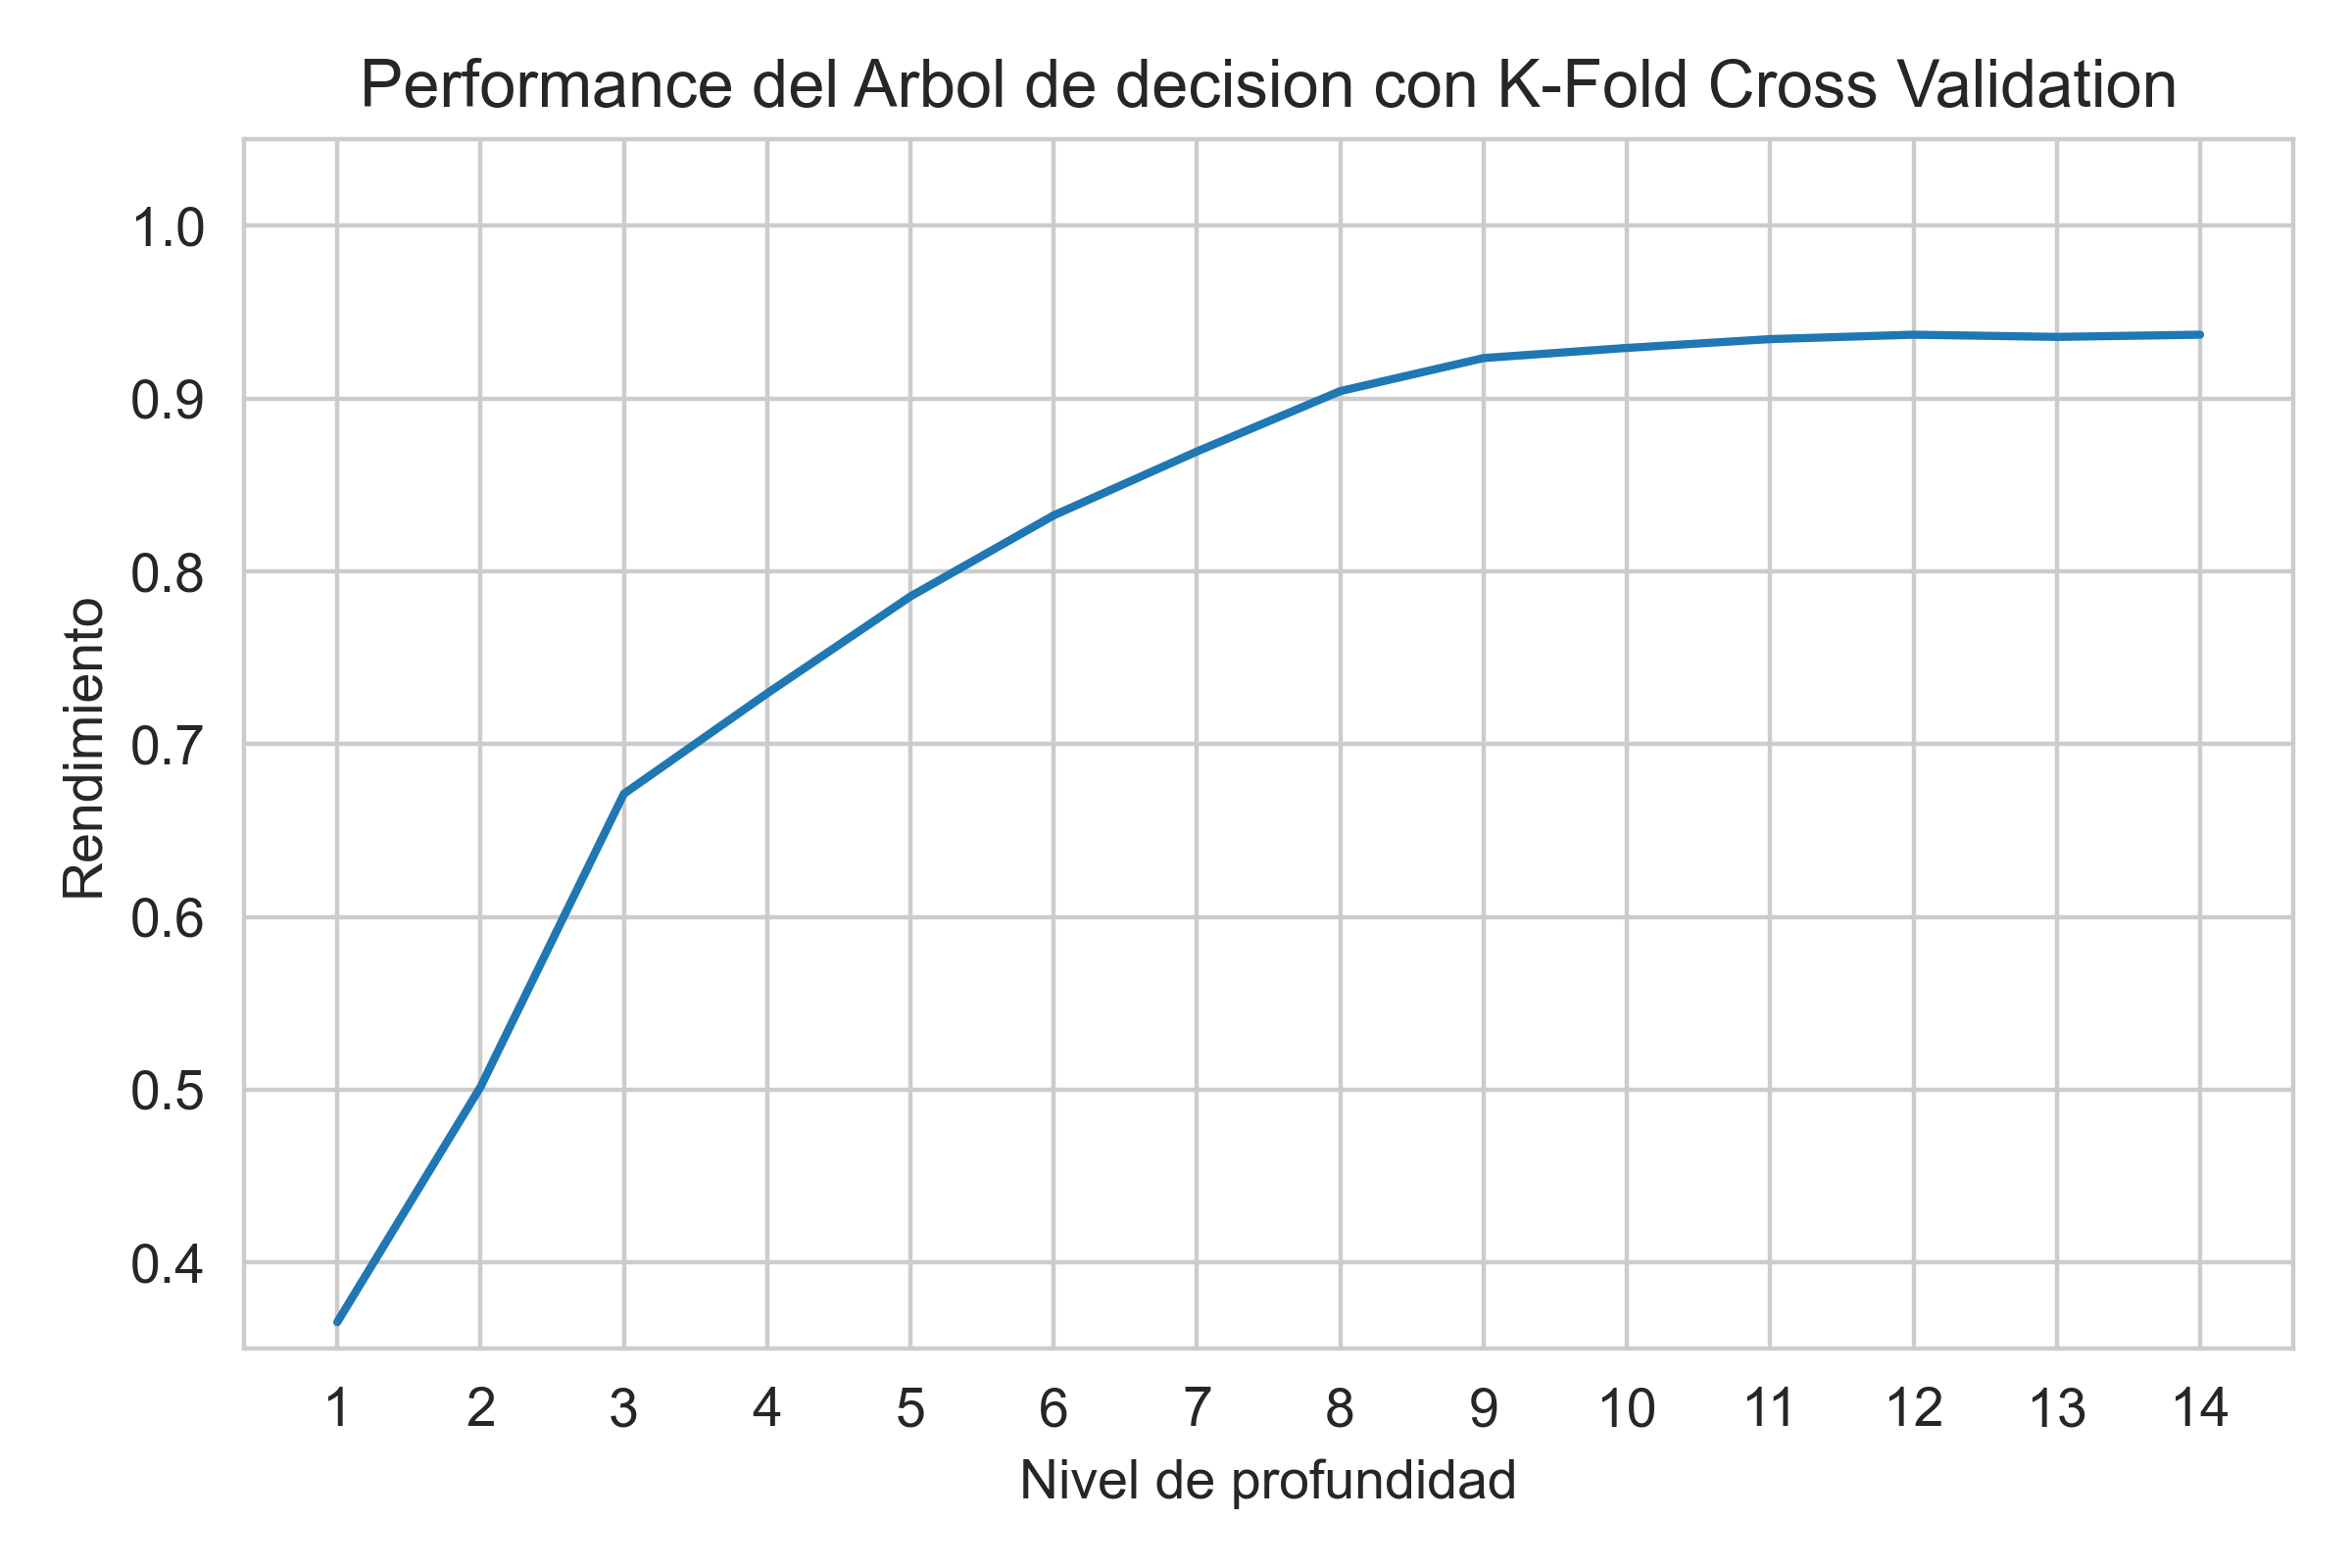
\includegraphics[width=1\linewidth]{Imagenes/KFold_prueba_arbol.png} 
		\caption{KFold}
		\label{fig:subfig1}
	\end{subfigure}
	\begin{subfigure}{0.5\textwidth}
		\includegraphics[width=1\linewidth]{Imagenes/tercer_Grafico_relacion.png}
		\caption{Comparacion entre ambos tests}
		\label{fig:subfig2}
	\end{subfigure}
	% OJO: el caption siempre va antes del label
	\label{fig:subfigs}
\end{figure}

A raiz, de los gráficos anteriores, pudimos notar que a partir de la altura 10, el modelo tiende a mantener su precisión. Por eso, nos quedaremos con estos valores e iremos testeando que ocurre combinandolos con otros hiperparametros. Para eso, realizamos un Grid Search tomando en cuenta los profundidades anteriormente nombradas, y los criterios, entropia y gini.

\newpage

\subsection{Grid Search}

En la imagen a continuación, la cual corresponde al Grid Search, podemos notar, primero que utlizar entropia es un poco mas eficiente que utilizar gini. Y, en segundo lugar, que el rendimiento entre profundidades practicamente no difiere. Por lo tanto, tomaremos aquel de menor profundidad en busca de tener un modelo mas simple. De esta manera, el modelo que escogeremos al final es un árbol de altura 10 con el criterio entropia. \vspace{0.05cm}

\begin{figure}[h]
  \centering
  \includegraphics[width=1\textwidth]{Imagenes/conclusion.png}
  \caption{Resultados Grid Search}
  \label{fig:Tabla 1}
\end{figure}

\subsection{Conclusión}

Para encontrar el mejor modelo, comenzamos testeando con el metodo de Kfold Cross Validation diferentes alturas, donde notamos que a partir de una altura 10 casi no variaba la precision de nuestro modelo. Luego, con esta información realizamos un Grid Search que incluia alturas entre 10 y 14 además de los criterios entropy y gini. A partir de este pudimos conlcuir que el modelo final es un árbol de altura 10 con el criterio entropia, el cual testeamos poniendo a prueba el modelo frente a los datos de test que separamos al principio de todo el proceso. En la página a continuación mostramos la matriz de confusión y los resultados finales.

\newpage

\subsection{Matris de Confusión y Test}

Para poder visualizar mejor donde acierta y donde no nuestro modelo, se recurrió a la matriz de confusión. Esta matriz es una herramienta que muestra de manera detallada cómo el modelo clasifica las muestras en cada una de las clases. Donde cada fila de la matriz representa la clase real, mientras que cada columna representa la clase predicha por el modelo.

\begin{figure}[ht]
  \centering
  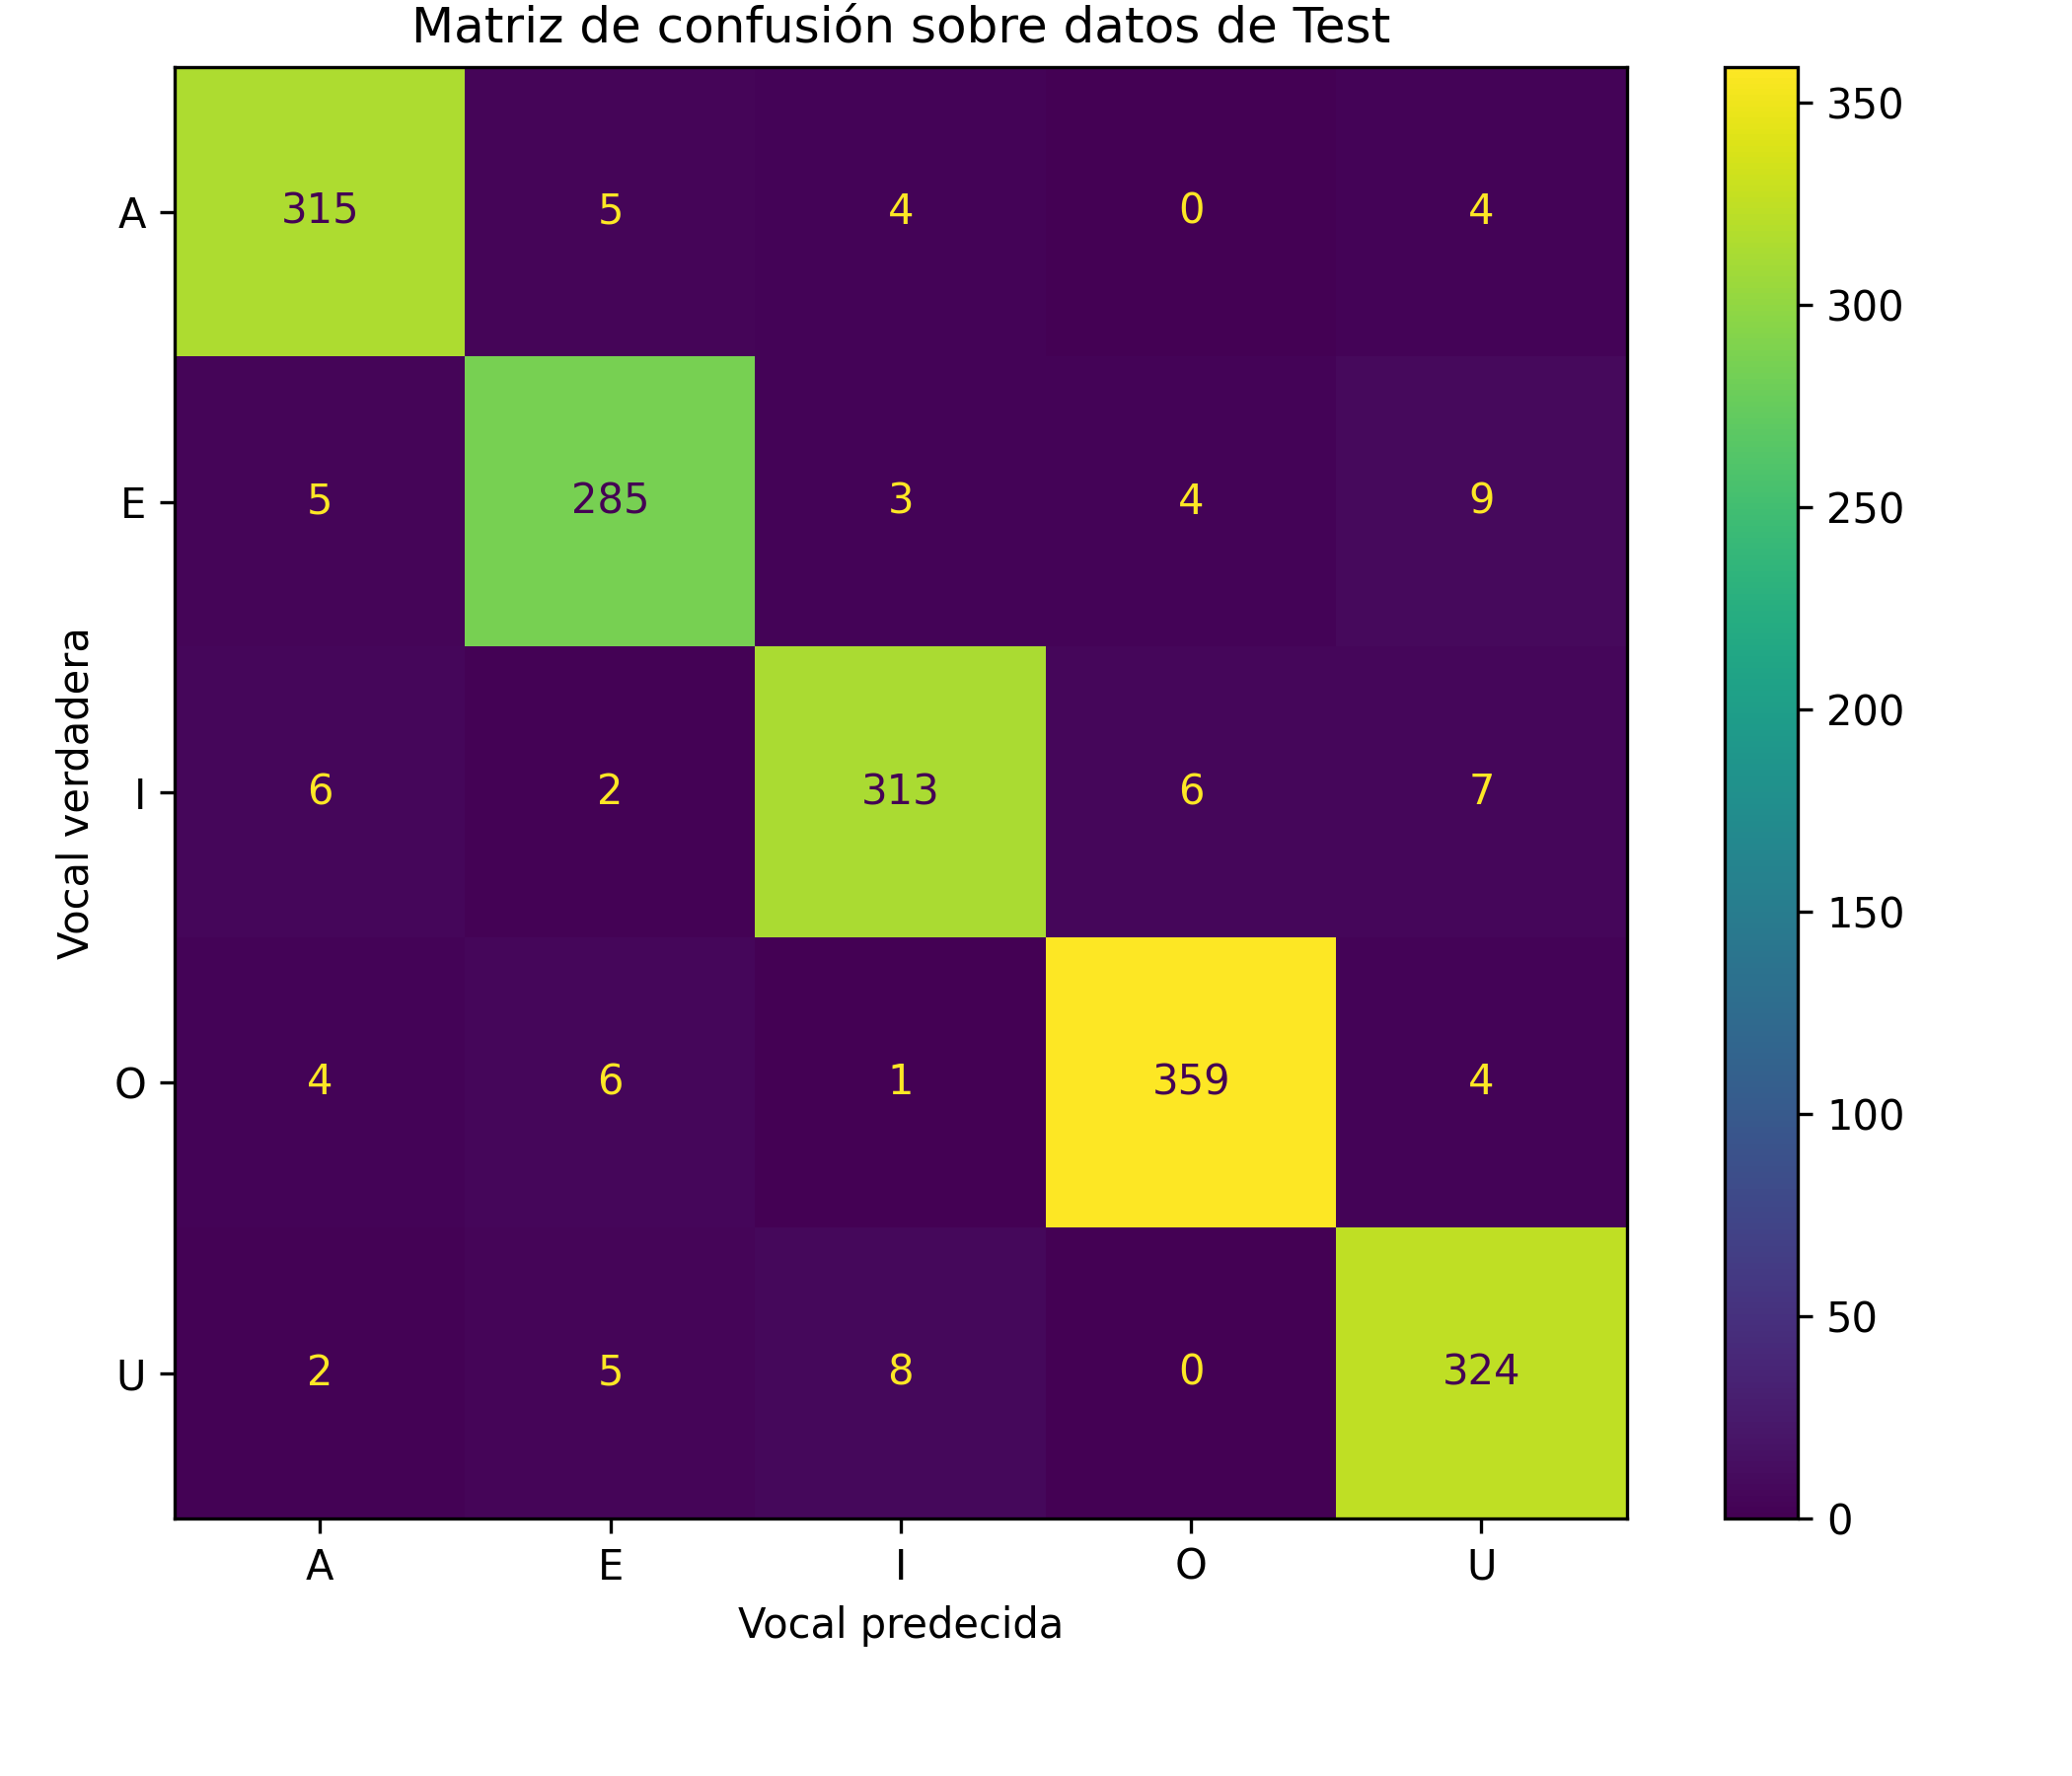
\includegraphics[width=0.6\textwidth]{Imagenes/matriz_confusion_arbol.png}
  \caption{Matriz de confusión}
  \label{fig:Tabla 1}
\end{figure}

Podemos notar, que nuestro modelo tiende a confundir las letras I y A por un lado, y las letras U e I. Sin embargo, tambien vemos que tiene un excelente desempeño mostrando una precisión del 0.9678.

Cabe aclarar, que tanto la matriz como la precisión fueron calculadas a partir de los datos de test, los cuales, habiamos reservado hasta este momento.

\end{document}
